\section{Resultados y discusión}
\subsection{Cómo leer los resultados}
Los resultados corresponden a una ejecución local sobre 56796 objetivos de prueba. Todos los modelos se evalúan sobre esas mismas posiciones. El bigrama presenta una configuración seleccionada por validación. Las filas principales de RNN y LSTM resumen tres semillas con contexto doce. Las comparaciones adicionales de longitud se presentan por separado porque tienen una sola semilla.

En pérdida y perplejidad, un valor menor es mejor. En top-1 y top-5, un porcentaje mayor es mejor. La desviación estándar describe la variación entre las tres ejecuciones de una arquitectura. No debe leerse como porcentaje de palabras incorrectas ni como una garantía de que cualquier nueva ejecución quedará dentro del intervalo escrito.

\begin{table*}[tb]
\caption{Comparación principal sobre 56796 objetivos. Las redes presentan media y desviación estándar muestral entre tres semillas.}
\label{tab:principal}
\centering
\begin{tabular}{lrrrr}
\toprule Modelo & NLL & Perplejidad & Top-1 léxico & Top-5 léxico\\\midrule
Bigrama & 4.453 & 85.93 & 2.82\% & 25.62\%\\
RNN & $4.325\pm0.005$ & $75.60\pm0.36$ & $7.23\pm0.56$\% & $26.58\pm0.08$\%\\
LSTM & $4.359\pm0.013$ & $78.15\pm1.05$ & $6.72\pm0.34$\% & $26.14\pm0.09$\%\\\bottomrule
\end{tabular}
\end{table*}

La Tabla~\ref{tab:principal} responde a varias preguntas. NLL y perplejidad muestran cómo se asignó probabilidad a las respuestas. Top-1 muestra la coincidencia del primer candidato. Top-5 muestra si la respuesta conocida se encontró dentro de los cinco primeros lugares de la distribución evaluada. Ninguna columna por sí sola describe toda la calidad de una experiencia de escritura.

\subsection{Comparación de perplejidad}
La RNN obtiene una perplejidad media de 75.60. La LSTM obtiene 78.15 y el bigrama 85.93. Bajo el mismo corpus y vocabulario, las redes mejoran al bigrama y la RNN presenta el menor valor. La diferencia entre la media LSTM y la media RNN es aproximadamente 2.55 puntos de perplejidad. Son puntos de esa medida, no puntos porcentuales de acierto.

La reducción relativa respecto al bigrama es aproximadamente 12.02\% para RNN y 9.05\% para LSTM. Se calcula restando la perplejidad de la red a la del bigrama y dividiendo por la del bigrama. Esa reducción no significa que se haya acertado ese porcentaje adicional de palabras. Informa un cambio relativo en perplejidad.

La desviación observada de LSTM, 1.05, es mayor que la de RNN, 0.36. En estas tres ejecuciones, los resultados de perplejidad de LSTM fueron más distintos entre sí. El tamaño del estudio es pequeño y conserva una sola partición de datos. No se realizó una prueba estadística de significación, por lo que se comunican las diferencias observadas sin convertirlas en una ley general sobre las arquitecturas.

\subsection{Resultados por semilla}
\begin{table*}[tb]
\caption{Ejecuciones individuales del estudio principal, contexto doce.}
\centering
\begin{tabular}{llrrrr}
\toprule Modelo & Semilla & NLL & Perplejidad & Top-1 (\%) & Top-5 (\%)\\\midrule
RNN & 17 & 4.320 & 75.21 & 7.88 & 26.57\\
RNN & 29 & 4.326 & 75.67 & 6.91 & 26.66\\
RNN & 43 & 4.330 & 75.92 & 6.91 & 26.50\\
LSTM & 17 & 4.367 & 78.82 & 6.87 & 26.04\\
LSTM & 29 & 4.343 & 76.94 & 6.32 & 26.20\\
LSTM & 43 & 4.365 & 78.69 & 6.95 & 26.19\\\bottomrule
\end{tabular}
\end{table*}

La tabla individual permite comprobar que una media resume valores distintos. También muestra que las métricas no siempre ordenan de la misma manera las ejecuciones de una arquitectura. La LSTM con semilla 29 tiene la menor perplejidad de su grupo principal, pero no el mayor top-1. Distribuir mejor probabilidad sobre los objetivos no obliga a que más objetivos ocupen exactamente el primer lugar.

La semilla 29 no se eligió para la demo por esta tabla de prueba. La selección utiliza la pérdida de validación conservada en los resúmenes de entrenamiento. Distinguir ambos criterios evita que la elección de la aplicación dependa de observar repetidamente el conjunto destinado a la evaluación final.

\subsection{Interpretación del acierto léxico}
El top-5 medio pasa de 25.62\% en el bigrama a 26.58\% en RNN y 26.14\% en LSTM. La mejora es aproximadamente 0.96 puntos porcentuales para RNN y 0.52 para LSTM. Aunque la perplejidad mejora en una proporción más visible, el cambio en la presencia de la palabra dentro de los cinco primeros lugares es pequeño.

La explicación es que una distribución puede asignar más probabilidad a una respuesta sin cambiar su posición lo suficiente para entrar en los cinco primeros lugares. También puede mejorar una respuesta que ya estaba dentro de esa lista y conservar el mismo acierto top-5. Las métricas observan aspectos distintos del resultado y por eso deben presentarse juntas.

El top-1 es 7.23\% para RNN y 6.72\% para LSTM, frente a 2.82\% del bigrama. Estos valores no justifican describir el prototipo como altamente preciso. La regla excluye UNK como acierto y conserva todos los objetivos en el denominador. En consecuencia, una alta frecuencia de objetivos desconocidos reduce las oportunidades de acertar una palabra concreta.

No se debe cambiar la definición de acierto después de ver que sus valores son bajos para que el sistema parezca mejor. La regla empleada se explica con claridad y se conserva. Se pueden proponer métricas adicionales en otro estudio, pero deben identificarse como adicionales y no mezclarse con las cifras obtenidas bajo la definición original.

\subsection{Lectura de la figura de comparación}
\begin{figure*}[tb]
\centering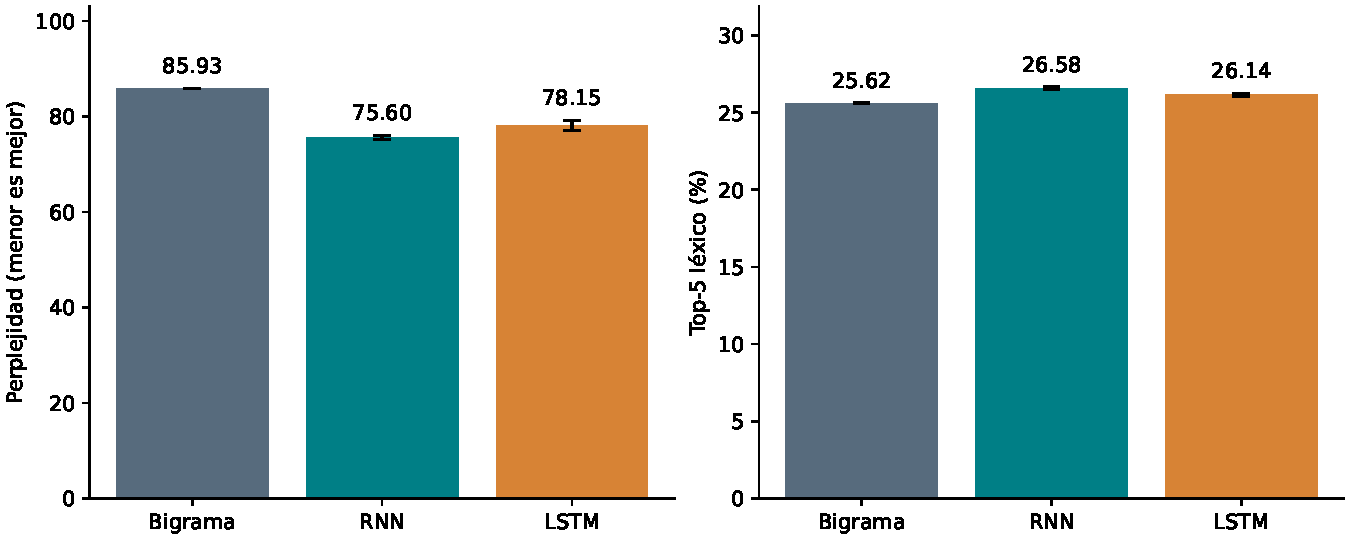
\includegraphics[width=.95\textwidth]{figuras/comparacion.pdf}
\caption{Perplejidad y top-5 de prueba. Las barras finas de las redes muestran desviación entre tres semillas, no incertidumbre sobre cualquier corpus.}
\label{fig:comparacion_nueva}
\Description{Dos gráficos de barras comparan bigrama, RNN y LSTM. La RNN tiene menor perplejidad y mayor top-5 en el protocolo ejecutado.}
\end{figure*}
La Figura~\ref{fig:comparacion_nueva} contiene dos gráficos. En ambos, el eje horizontal identifica los modelos. En el gráfico de la izquierda, el eje vertical corresponde a perplejidad; una barra más baja representa un resultado mejor. En el de la derecha, el eje vertical representa porcentaje top-5; una barra más alta representa mayor acierto.

Las pequeñas marcas negras encima de las barras de las redes muestran la variación entre semillas. Su poca altura en top-5 indica que los porcentajes de esas tres ejecuciones estuvieron próximos. No expresa ausencia de errores en las palabras: un modelo puede mantener resultados parecidos entre semillas y seguir acertando una proporción limitada de objetivos.

La figura facilita comparar visualmente los valores, mientras que las tablas permiten consultar números concretos. Ambas provienen de los mismos registros. No son dos experimentos independientes. Los colores distinguen modelos y no representan clases gramaticales, lenguas ni conjuntos de datos.

\subsection{Curvas de aprendizaje}
\begin{figure*}[tb]
\centering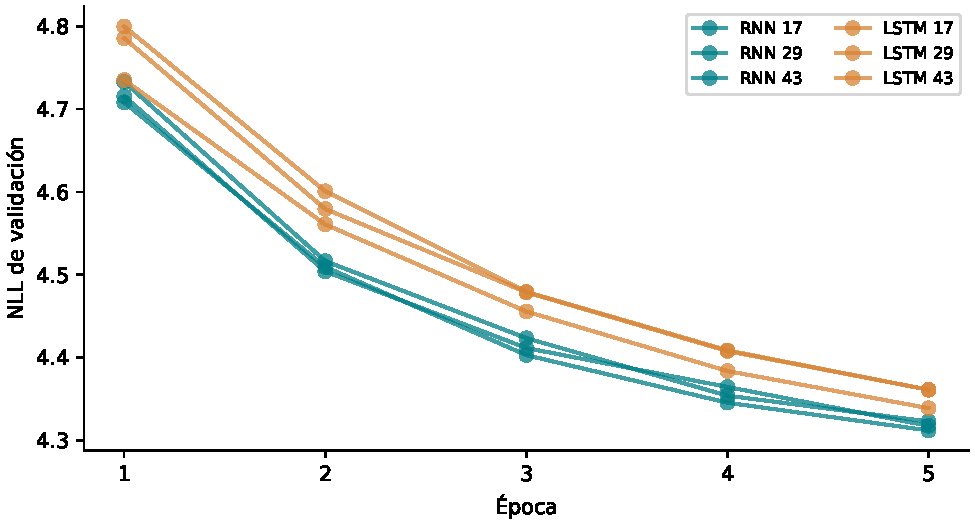
\includegraphics[width=.78\textwidth]{figuras/aprendizaje.pdf}
\caption{Pérdida de validación durante las cinco épocas del estudio principal. Cada línea corresponde a una arquitectura y una semilla.}
\label{fig:aprendizaje_nueva}
\Description{Seis curvas muestran una disminución de pérdida de validación durante las cinco épocas para RNN y LSTM.}
\end{figure*}
La Figura~\ref{fig:aprendizaje_nueva} usa el eje horizontal para indicar la época y el vertical para indicar NLL de validación. Cada punto resume todos los objetivos de validación de una época. Una línea une los cinco puntos de una misma ejecución. Las etiquetas 17, 29 y 43 son semillas, no números de palabras ni cantidades de capas.

Las curvas descienden a lo largo del entrenamiento observado. Esto indica que las versiones sucesivas asignaron mejor probabilidad a los objetivos de validación en ese tramo. No demuestra que el modelo haya alcanzado su mejor resultado posible. Para examinar qué ocurre con más épocas sería necesario un experimento adicional que no ajuste decisiones a partir de la prueba ya utilizada.

La figura representa validación, no prueba. Esta distinción es importante porque validación interviene en la selección del modelo guardado. Utilizar una curva de prueba para elegir la época mezclaría la selección con la evaluación final. El programa mantiene separadas esas dos funciones.

\subsection{Seguimiento de una ejecución completa}
Para concretar la lectura de las curvas, se presenta la ejecución LSTM con contexto doce y semilla 29, correspondiente al modelo seleccionado para la demo. La tabla siguiente muestra sus cinco épocas. Los datos proceden del historial guardado durante entrenamiento y se redondean únicamente para su presentación.

\begin{table*}[tb]
\caption{Historial observado de LSTM, contexto doce, semilla 29.}
\centering
\begin{tabular}{rrrrr}
\toprule Época & NLL entrenamiento & NLL validación & PPL validación & Top-5 validación (\%)\\\midrule
1 & 5.291 & 4.735 & 113.89 & 22.96\\
2 & 4.734 & 4.561 & 95.66 & 24.68\\
3 & 4.557 & 4.456 & 86.10 & 25.30\\
4 & 4.431 & 4.384 & 80.13 & 26.19\\
5 & 4.338 & 4.339 & 76.61 & 26.49\\\bottomrule
\end{tabular}
\end{table*}

La pérdida de validación disminuye de 4.735 a 4.339 en las épocas registradas. La perplejidad también disminuye y el top-5 aumenta. En esta ejecución, la quinta época tiene la menor NLL de validación, por lo que es la versión conservada. La tabla permite justificar esa selección sin recurrir al resultado final de prueba.

La pérdida de entrenamiento se acumula mientras el modelo está aprendiendo. Dentro de una época, los parámetros cambian después de cada lote. En cambio, la pérdida de validación se obtiene al terminar la época, con la versión de parámetros de ese momento. Por esta razón, no se deben interpretar sus valores como si fueran dos evaluaciones simultáneas de un modelo idéntico sobre datos intercambiables.

También cambia el modo de operación: dropout está activo mientras se entrena y se desactiva al evaluar. Las particiones poseen sus propias palabras y frecuencias. Una diferencia entre columnas, por sí sola, no demuestra que exista un error ni permite cuantificar toda la capacidad de generalización. Para interpretar sobreajuste se necesita examinar la evolución y el diseño, no exigir igualdad exacta entre pérdidas.

La primera época ya contiene muchas actualizaciones. Su resultado no representa una red completamente sin entrenamiento. Del mismo modo, la quinta fila no corresponde a una nueva arquitectura: conserva las mismas dimensiones y cambia los parámetros que aprendieron durante las pasadas anteriores. Los puntos de una curva describen versiones sucesivas de una ejecución, mientras que las semillas describen ejecuciones distintas.

El top-5 de validación de la última fila es aproximadamente 26.49\%. El top-5 de prueba de ese mismo modelo es aproximadamente 26.20\%. La diferencia responde a conjuntos distintos. No se reemplaza la cifra de prueba por la de validación para presentar un porcentaje mayor. Tampoco se promedian ambas particiones, porque sus funciones dentro del protocolo son diferentes.

La perplejidad de validación de esa fila es 76.61, frente a 76.94 en prueba para la ejecución seleccionada. Estos dos valores tampoco deben confundirse con la media de 78.15 de las tres LSTM principales. Existen tres niveles de lectura: una versión por época en validación, una ejecución seleccionada evaluada en prueba y un promedio de varias ejecuciones. Informar a cuál corresponde cada número evita aparentes contradicciones.

El seguimiento numérico complementa la figura y permite repetir una comprobación sencilla: localizar la menor pérdida de validación en el historial, consultar la época guardada del modelo y confirmar su identidad. No exige volver a entrenar para comprobar lo que ya quedó registrado. Una nueva ejecución independiente sería una comprobación adicional de reproducibilidad, distinta de verificar la coherencia interna de estos archivos.

\subsection{Efecto de la longitud de contexto}
\begin{table*}[tb]
\caption{Comparación exploratoria de contextos con semilla 17.}
\centering
\begin{tabular}{lrrrr}
\toprule Modelo & Contexto máximo & Perplejidad & Top-1 (\%) & Top-5 (\%)\\\midrule
RNN & 4 & 75.49 & 7.64 & 26.50\\
RNN & 12 & 75.21 & 7.88 & 26.57\\
RNN & 24 & 75.73 & 7.74 & 26.54\\
LSTM & 4 & 78.30 & 6.69 & 26.05\\
LSTM & 12 & 78.82 & 6.87 & 26.04\\
LSTM & 24 & 78.46 & 7.05 & 25.99\\\bottomrule
\end{tabular}
\end{table*}

En RNN, el contexto doce obtiene menor perplejidad que cuatro y veinticuatro para la semilla mostrada. En LSTM, el contexto cuatro obtiene menor perplejidad que doce y veinticuatro en esta comparación. No se observa que aumentar el contexto produzca una mejora continua de todas las métricas.

El resultado debe interpretarse con cautela porque cada contexto adicional tiene una sola semilla. No permite distinguir con suficiente detalle el efecto de la longitud de otras variaciones de entrenamiento. Tampoco prueba que una LSTM no pueda aprovechar dependencias largas: la tarea utiliza ventanas relativamente cortas, un presupuesto breve y texto natural cuya información relevante no se controló por distancia.

La fila con contexto doce de esta tabla corresponde únicamente a la semilla 17. No debe sustituirse por la media de tres semillas de la tabla principal sin avisar, porque se mezclarían niveles de resumen. Esta diferencia explica que aparezcan 75.21 y 78.82 aquí, mientras que la comparación principal presenta 75.60 y 78.15.

\subsection{Cobertura del vocabulario}
De los 56796 objetivos de prueba, 12033 se representan como UNK. Esto equivale aproximadamente a 21.19\%. Las posiciones restantes, 44763, corresponden a entradas identificables. Incluso si el modelo acertara todas esas posiciones conocidas, no podría superar aproximadamente 78.81\% de acierto léxico con la regla actual y sin ampliar su capacidad de producir palabras.

Ese límite no describe el acierto alcanzado, sino un máximo impuesto por la representación. El top-5 real es mucho menor. La cobertura explica una parte de la dificultad, pero no todas las predicciones incorrectas: también existen palabras conocidas que el modelo ordena fuera de los primeros lugares.

La perplejidad trata de otra manera estas posiciones porque utiliza UNK como objetivo interno. El modelo puede asignar probabilidad a esa categoría y recibir una pérdida limitada aunque no distinga el término original. Por eso la perplejidad de un vocabulario reducido no debe compararse sin más con la de otro sistema que represente todas las palabras de forma distinta.

\subsection{Cantidad de parámetros}
La RNN tiene 346296 parámetros y la LSTM 368184. La diferencia es 21888, aproximadamente 6.32\% respecto a la RNN. En ambas arquitecturas, la representación de palabras aporta 144000 parámetros y la proyección de salida aporta 195000. La parte recurrente contiene 7296 en RNN y 29184 en LSTM.

La diferencia total es menor de lo que podría esperarse al observar cuatro transformaciones recurrentes en LSTM, porque embedding y salida ocupan una parte grande del total y son iguales en ambas redes. Esto ayuda a interpretar el tamaño del modelo. Una mayor cantidad de parámetros no es sinónimo de mayor acierto y no describe por sí sola cuántas operaciones se realizan en cada consulta.

\begin{table*}[tb]
\caption{Distribución de parámetros de la configuración usada.}
\centering
\begin{tabular}{lrr}
\toprule Componente & RNN & LSTM\\\midrule
Embedding & 144000 & 144000\\
Parte recurrente & 7296 & 29184\\
Proyección final & 195000 & 195000\\\midrule
Total & 346296 & 368184\\\bottomrule
\end{tabular}
\end{table*}

\subsection{Tiempos de ejecución}
El tiempo medio de entrenamiento de las tres ejecuciones principales fue 78.17 segundos para RNN y 107.44 segundos para LSTM. Las cinco épocas y las evaluaciones de validación forman parte de ese tiempo registrado. La comparación utiliza CPU y dos hilos. No se interpreta como una garantía de duración en cualquier computadora.

Se midió también la duración del cálculo de una predicción con lote de un ejemplo, después de diez calentamientos y sobre cien consultas. La mediana indica el valor central de los tiempos ordenados y el percentil 95 indica el valor por debajo del cual se encuentra aproximadamente el 95\% de las mediciones. Estas mediciones excluyen carga del archivo, tokenización y escritura de salida.

La demo vuelve a cargar el modelo en cada consulta, de modo que la espera que observa la persona incluye actividades adicionales. Por eso el tiempo del cálculo interno no se presenta como tiempo total de respuesta de la aplicación. Para una evaluación de uso real se tendría que medir el recorrido completo y controlar la carga del equipo.

\subsection{Ejemplos observados en la demostración}
Con entrada vacía, el programa procesa la señal de inicio. La primera sugerencia registrada es ``el'' con aproximadamente 14.21\%. Le siguen ``la'', ``en'', ``los'' y ``pero''. La probabilidad de UNK es aproximadamente 10.95\%. Este caso permite comprobar que una entrada sin palabras se trata de forma definida y no produce una operación sin elementos.

Para ``el presidente del gobierno'', las sugerencias registradas son ``de'', ``del'', ``vasco'', ``es'' y ``se''. La palabra ``de'' recibe aproximadamente 13.77\%; UNK recibe 10.61\%. La entrada no contiene palabras desconocidas. Aun así, el programa no conoce la continuación que pretende escribir una persona y presenta varias opciones en lugar de una afirmación de corrección única.

\begin{table*}[tb]
\caption{Salida observada para ``el presidente del gobierno''. Las probabilidades conservan su valor dentro de la distribución completa.}
\centering
\begin{tabular}{lrr}
\toprule Candidata & Posición visible & Probabilidad aproximada\\\midrule
de & 1 & 13.77\%\\
del & 2 & 7.35\%\\
vasco & 3 & 3.00\%\\
es & 4 & 1.97\%\\
se & 5 & 1.97\%\\\bottomrule
\end{tabular}
\end{table*}

Para ``la universidad de'', la primera sugerencia es ``la'', con aproximadamente 10.74\%, y UNK recibe 20.02\%. La lista incluye la categoría numérica. El ejemplo muestra que una entrada completamente conocida no asegura que la salida resulte suficientemente específica para el uso esperado. La red puede favorecer términos generales y no producir el nombre concreto que una persona espera.

En ``los estudiantes de software'', la palabra ``software'' aparece como desconocida. La primera sugerencia es ``de'', con aproximadamente 7.53\%, y UNK recibe 22.05\%. Este resultado se relaciona con la lista de vocabulario utilizada, no con la afirmación de que el término no exista en español técnico. El programa solo informa que no dispone de una entrada propia para esa forma.

En ``Riobamba ESPOCH Chimborazo'', las tres formas normalizadas son desconocidas. La primera sugerencia es ``de'', con aproximadamente 5.07\%, y UNK recibe 24.64\%. El caso ayuda a mostrar la diferencia entre disponer de un modelo en español y reconocer vocabulario local concreto. No se puede atribuir a estas salidas un conocimiento comprobado de la ciudad o la institución.

Los ejemplos de demo se seleccionaron para explicar comportamientos. No constituyen una muestra aleatoria de todas las consultas posibles. Tampoco tienen una única palabra de referencia que permita contarlos automáticamente como acierto o error. La evaluación cuantitativa utiliza el conjunto de prueba; los ejemplos permiten examinar cómo se presenta el resultado a una persona.

\subsection{Qué permite concluir la comparación}
Las redes obtuvieron mejor perplejidad que el bigrama bajo el protocolo usado. La RNN obtuvo el mejor promedio principal de las métricas informadas. La mejora top-5 respecto al bigrama fue menor de un punto porcentual. Estas son conclusiones apoyadas por los valores registrados.

Una posible explicación de que LSTM no obtenga ventaja es que el tamaño de la muestra, las ventanas y las cinco épocas no favorezcan un aprovechamiento suficiente de su mecanismo de memoria. Sin embargo, el estudio no modifica cada factor de manera independiente para comprobar esa explicación. Debe presentarse como posibilidad, no como causa demostrada.

Las referencias sobre LSTM describen capacidades y resultados en otros escenarios. No obligan a que toda implementación local supere a una RNN simple. Conservar un resultado distinto de la expectativa permite mostrar una práctica de investigación adecuada: describir el experimento, informar los datos y limitar la conclusión a lo que se midió.

\subsection{Limitaciones del estudio}
La primera limitación es el vocabulario reducido y su alta proporción de desconocidas. La segunda es el dominio periodístico, que no representa todos los usos del español. La tercera es el presupuesto de entrenamiento: cinco épocas permiten una comparación concreta, pero no garantizan que cada arquitectura haya alcanzado su mejor configuración.

También existen límites de comparación. Usar la misma tasa de aprendizaje no significa que sea igualmente adecuada para ambas redes. Utilizar el mismo tamaño oculto no iguala cantidad de parámetros. Repetir tres semillas no sustituye repetir el experimento con varios corpus o divisiones. Estos puntos no invalidan las mediciones; delimitan la pregunta que realmente respondieron.

La separación por documento y la eliminación de duplicados exactos reducen riesgos de coincidencia entre datos, pero no eliminan noticias similares. La evaluación automática tampoco mide si una persona acepta una sugerencia. Un despliegue real necesitaría valorar errores de escritura, tiempos completos de respuesta, pertinencia de candidatos y comportamiento con vocabulario del entorno de uso.

\subsection{Relación con el propósito educativo}
La práctica permite seguir una cadena verificable: texto original, preparación, ejemplos, arquitectura, entrenamiento, evaluación y sugerencias. Esa relación es más importante para comprender el tema que memorizar una cifra aislada. Un integrante debe poder explicar cómo se obtiene el resultado y qué decisión cambiaría si se modifica una condición del experimento.

Las preguntas técnicas de la defensa pueden responderse a partir de esa cadena. La memoria se explica en el estado y la celda; las compuertas, en la actualización LSTM; la calidad predictiva, en las métricas; y la reproducibilidad, en las configuraciones y datos guardados. No es necesario introducir arquitecturas ajenas al tema para justificar el alcance del programa presentado.
